% Chapter Template

\chapter{Results}\label{Results} % for referencing this chapter elsewhere, use \ref{Results}

%----------------------------------------------------------------------------------------
%	SECTION 1
%----------------------------------------------------------------------------------------

\section{NMF Signatures}

The NMF produces two factorized matrices, \(H\) and \(W\). Among them, \(H\) matrix is the one that relates the epigenetic marks to the signatures, giving a \(7 \times 11\) array. From this matrix, we can study the combinatorial relations between the epigenetic modifications. One important aspect to bear in mind is that the signatures which yield from the method do not come off in the same order. This is due to the random initialization of the matrices. Therefore, referring to particular signature numbers in the following lines is just used for comparison purposes. A good way to compare the \(H\) matrix outcome is by analyzing the values in it using a heatmap plot. In order to relate the signatures from the different cell tissues, correlation between their values was used.

\begin{figure}[h!]
    \centering
    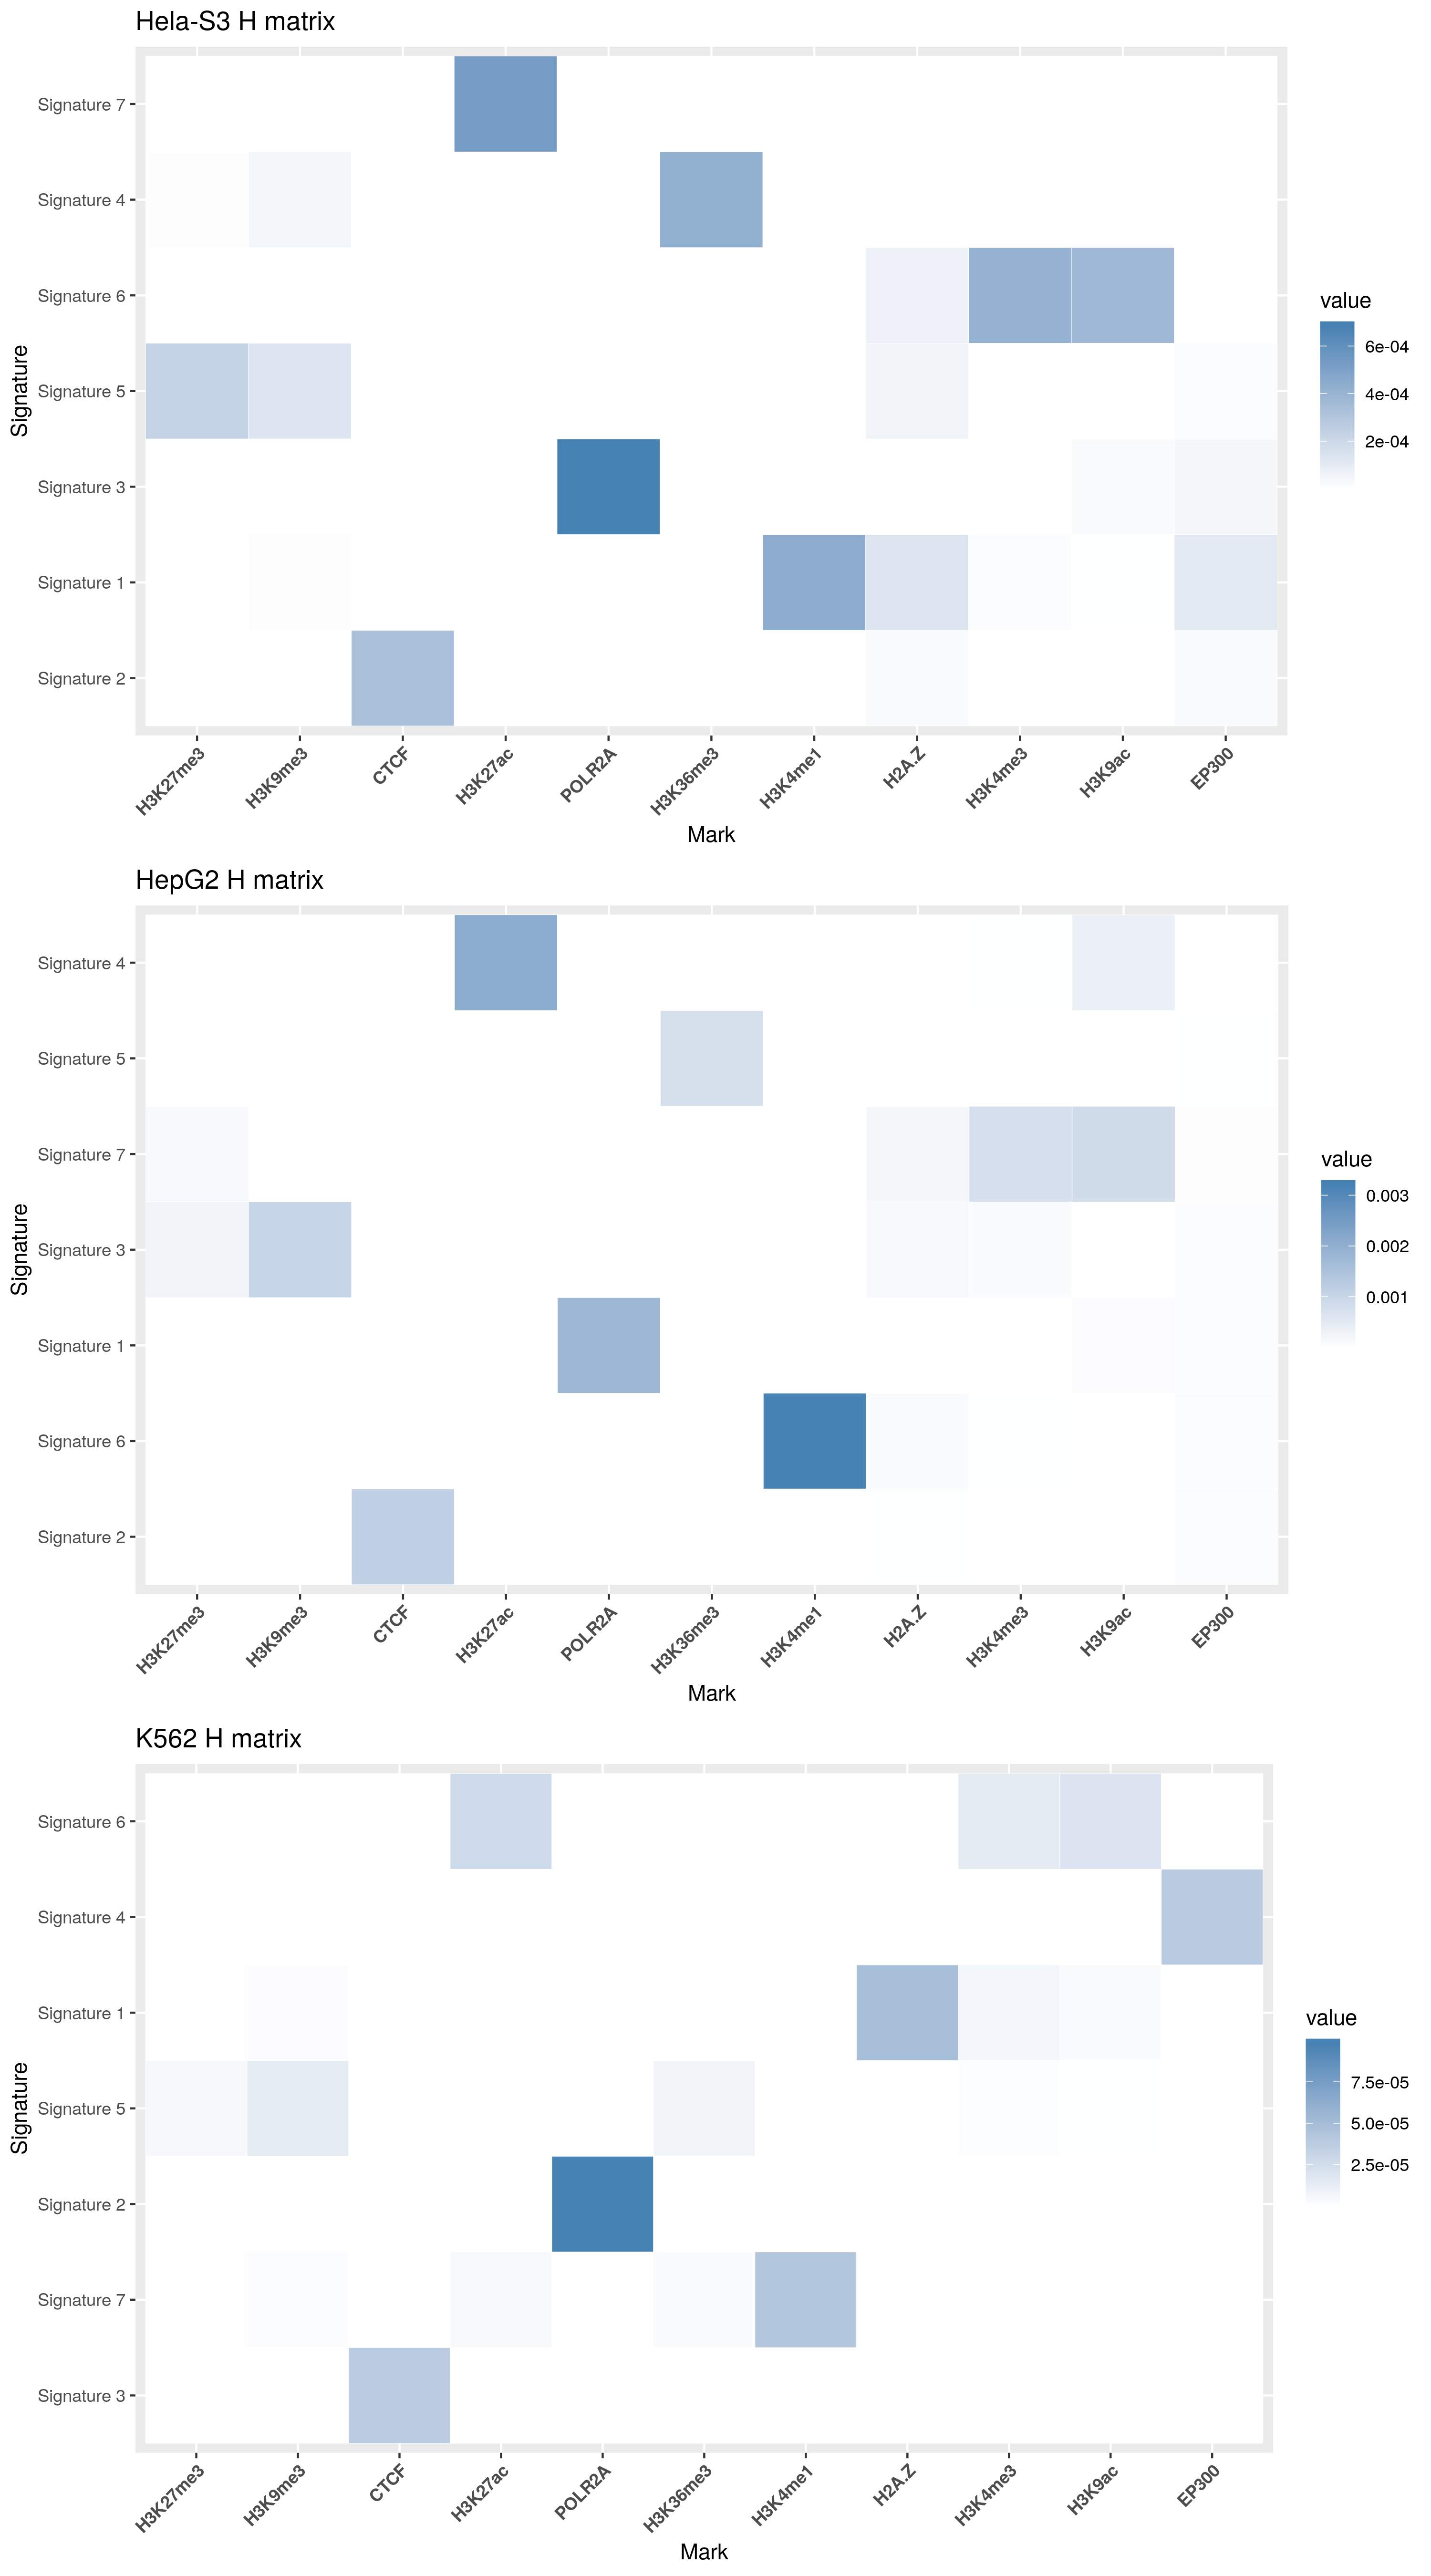
\includegraphics[width=0.8\textwidth]{Figures/NMF/vert_comb.png}
    \caption[Heatmap of the obtained H matrices]{\textbf{Heatmap of the obtained H matrices}. Heatmap of the \(W\) matrix weights obtained from NMF algorithm. From top to botton we see the results for the Hela-S3 cell line, HepG2 cells and K562. The signatures were ordered by correlation, which facilitate the comparison between plots.}
    \label{fig:H_heatmaps}
\end{figure}

Figure~\ref{fig:H_heatmaps} shows the \(H\) matrix results for the three cell lines analyzed. The arrangement of the signatures was decided according in order to correspond to the one shown in \cite{Gandolfi2017}. As we can see, there are numerous coincidences between the heatmaps. Assuming we related the signatures correctly, we can adopt the same `genomic labels' for the signatures in the following order from top to bottom: (1) `Active Promoter', (2) `Repressed Chromatin', (3) `Transcription Initiation', (4) `Repressed Regulatory Regions', (5) `Gene Body Transcription',  (6) `Enhancer Regions' and (7) `Regulatory Elements'.

\begin{enumerate}
    \item The `Active Promoter' signature shows a predominance of H3K27ac modification, associated with a higher activation of the gene expression (acts as an active enhancer mark). HepG2 and K562 show in addition importance of the H3K9ac modification, also correlated with active promoters. H3K4me3 is an activation-related modification which also appears to be important in K562 tissue.
    \item In the `Repressed Chromatin' signature in contrast, the predominant marks in Hela-S3 are H3K36me3 and to a lesser extent H3K9me3. H3K36me3 and H3K9me3 are both known to be implicated in the repression of aberrant trancription \cite{Bartke2010}. It is noticeable how in the cancer cells analyzed in this report, it is more predominant the presence of H3K36me3 than H3K9me3 while it is the other way around for the IMR90 cell line. H3K36me3 is known for serving as a mark for the histone descetylases (HDACs) to act in the DNA. This can be related with the amplified action of the HDACs seen in cancer cells.
    \item `Transcription Initiation' includes the presence of H2A.Z, H3K4me3 and H3K9ac, all of them activators when they are localized close to the promotors.
    \item `Repressed Regulatory Regions' signature includes H3K27me3 as in IMR90 but in the cancer cells it is also important H3K9me3, in any case, both related with heterochromatic regions.
    \item `Gene Body Transcription' includes a dominant presence of DNA-directed RNA polymerase II subunit gene (POLR2A).
    \item In the `Enhancer Regions' signature, H3K4me1 stands out for Hela-S3, HepG2 and K562. H3K4me1 is seen as a ``window of opportunity'' for the enhancer activation by modulating nucleosomal mobility through the H2A.Z-containing nucleosomes. This process provokes the chromatin structure to be more dynamic, enhancing the Transcription Factor accessibility. This is consistent with the co-occurrenceof H2A.Z in this signature.
    \item Last, `Regulatory Elements' signature comprise the Transcriptional repressor CTCF.
\end{enumerate}

\section{Signature distribution along the genome}

\begin{figure}[h!]
    \centering
    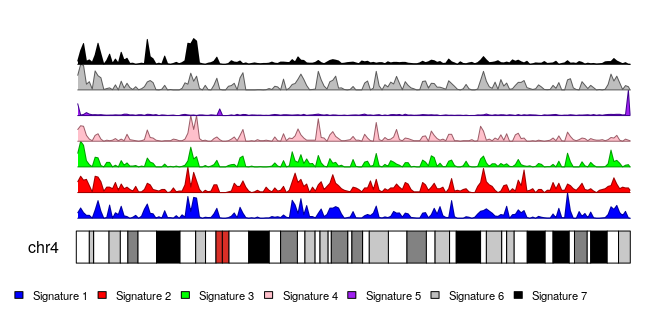
\includegraphics[width=\textwidth]{Figures/cover/chr4.png}
    \caption[Signatures density in chromosome 4]{\textbf{Signatures density in chromosome 4}. Representation of the chromosome 4 and overlay with the density distribution of the signatures. Signature 1 (Active Promoter) is represented in blue, Signature 2 (Repressed Chromatin) in red, Signature 3 (Transcription Initiation) in green, Signature 4 (Repressed Regulatory Regions) in pink, Signature 5 (Gene Body Transcription) in purple, Signature 6 (Enhancer Regions) in grey and Signature 7 (Regulatory Elements) in black}
    \label{fig:chr4}
\end{figure}

The second factorized matrix is the \(W\) matrix, which relates the signatures with the bins and thus with the genome location. In this way, we can associate each of the bins their prevailing signature. Each bin got assigned the signature for which the weight was highest. This been done, the distribution of the signatures along the genome can be represented using a density plot. Figure \ref{fig:W_density} shows an example representation of the signature location along the chromosomes.

\begin{sidewaysfigure}[ht]
    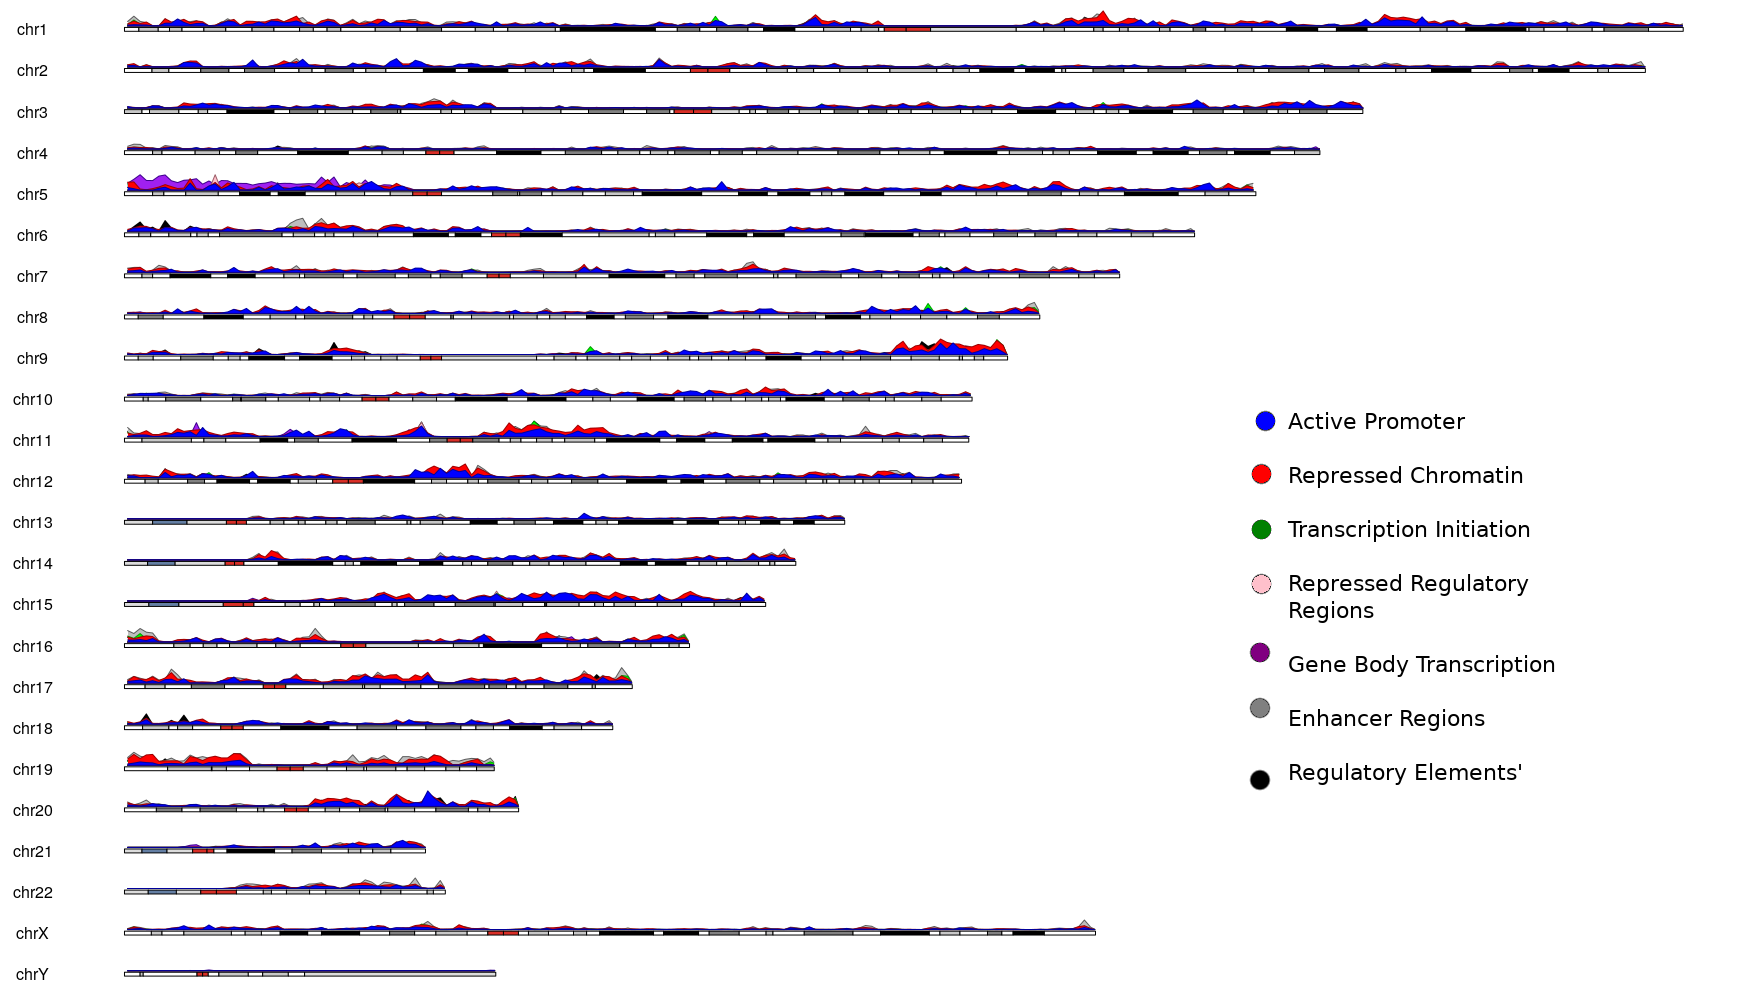
\includegraphics[width=\textwidth]{Figures/cover/signatures_density.png}
    \caption[Signatures density along the chromosomes]{\textbf{Signatures density along the chromosomes}. Figure description. Lots of things. Lots of things. Lots of things. Lots of things.Lots of things. Lots of things. Lots of things. Lots of things.Lots of things. Lots of things. Lots of things. Lots of things.}
    \label{fig:W_density}
\end{sidewaysfigure}

\medskip

Taking chromosome 4 as an example, we can better see the distribution of the signatures in Figure~\ref{fig:chr4}. In this case, Hela-S3 results are presented and we can observe a few patterns:

\begin{itemize}
    \item All the signatures but 5 (Gene Body Transcription) follow a similar distribution along the chromosome 4.
    \item Signatures 1 (Active Promoter), 3 (Transcription Initiation), 4 (Repressed Regulatory Regions) and 6 (Enhancer regions) share a even similar profile. Being these signatures related to the gene activation, the observation for chromosome 4 go along with the involved biological processes.
    \item In points where the signatures described in the last point are the lowest, signature 2 (Repressed Chromatin) presents peaks.
    \item Signature 5 (Gene Body Transcription) ilustrates a generaly low occurrence of bins assigned to the group in chromosome 4. Moreover, we see remarkable maximum peaks in the beginning and the end of the chromosome as well as the centromere.
    \item For signature 7 (Regulatory Elements), it looks like it is more dominant in the left arm of the chromosome 4.
\end{itemize}
